\section{Results and discussion（结果与讨论）}
\label{sec:results}

\subsection{Accuracy across benchmark problems（跨算例的精度）}
\label{sec:accuracy}

六个算例覆盖了不同的主场、算子与参数化（表~\ref{tab:cases}）。Couette--Graetz 与共轭传热以温度为主场，算子线性、非对称，后者含导热率跳变的流固界面；方腔自然对流、混合对流与多孔方腔以流函数为主场，流热双向耦合，分别由浮力、剪切与浮力、多孔阻力主导；后台阶为开口通道中的分离流动，几何参数改变回流区的位置与尺度。除方腔自然对流取 12 个快照外，其余算例只用训练区四角的 4 个快照及其灵敏度。

\begin{figure}[H]
\centering
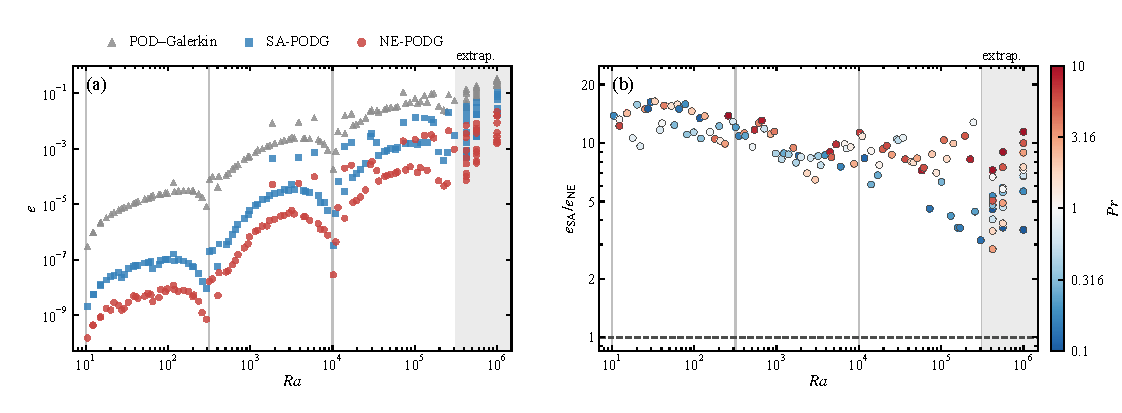
\includegraphics[width=\textwidth]{Fig_03.pdf}
\caption{六个算例默认快照预算下的精度。(a) POD--Galerkin、SA-PODG 与 NE-PODG 主场误差 $e$ 的分布：细线为最小值到最大值，粗段为四分位区间，点为中位数（实心为内插，空心为外推），$\times$ 为该空间内没有 Galerkin 解的工况；(b) 两种方法都解出的工况上逐工况的误差比 $e_{\mathrm{SA}}/e_{\mathrm{NE}}$，横线为中位数。}
\label{fig:accuracy}
\end{figure}

SA-PODG 的主场误差中位数比 POD--Galerkin 低 3.6--86 倍，NE-PODG 在所有算例的内插与外推测试上进一步降低误差（图~\ref{fig:accuracy}(a)）。两种方法都解出的工况上，逐工况的误差比 $e_{\mathrm{SA}}/e_{\mathrm{NE}}$ 均不小于 1（图~\ref{fig:accuracy}(b)）。误差比的中位数在 Couette--Graetz 上为 27.1（内插）与 21.3（外推），共轭传热为 25.2 与 7.58，方腔自然对流为 9.93 与 5.64，混合对流为 5.66 与 6.37，多孔方腔为 4.82 与 4.59，后台阶为 2.16 与 2.26：线性算例的增益最大，非线性流热耦合算例居中，后台阶最小。NE-PODG 同时压低误差分布的尾部，后台阶内插的最大误差由 33.1\% 降为 7.02\%，方腔自然对流外推由 10.4\% 降为 2.14\%，混合对流外推由 16.9\% 降为 3.06\%。后台阶外推的 27 个工况中，SA-PODG 在 2 个工况上没有 Galerkin 解，Levenberg--Marquardt 迭代停在相对残差 $2.4\times10^{-2}$ 与 $6.8\times10^{-2}$ 处；NE-PODG 在这两个工况上收敛，误差为 4.32\% 与 4.04\%。

\begin{table}[H]
\centering
\caption{六个算例默认快照预算下传热量的相对误差（\%）。统计只含该方法解出的工况。$\overline{Nu}$ 为平均 Nusselt 数（方腔类算例为冷壁，后台阶为受热壁）；局部 $Nu$ 为沿受热壁（Couette--Graetz）或四个界面位置（共轭传热）的最大相对误差；$Q$ 为界面总热流。}
\label{tab:heat}
\footnotesize
\setlength{\tabcolsep}{3pt}
\begin{tabular}{lllcccc}
\toprule
 & & & \multicolumn{2}{c}{Interpolation} & \multicolumn{2}{c}{Extrapolation} \\
\cmidrule(lr){4-5}\cmidrule(lr){6-7}
Problem & Output & Method & median & max & median & max \\
\midrule
Natural convection & $\overline{Nu}$ & POD-G & $2.60\times10^{-4}$ & 0.948 & 2.84 & 8.91 \\
 &  & SA-PODG & $3.49\times10^{-6}$ & 0.0881 & 0.0792 & 1.22 \\
 &  & NE-PODG & $2.84\times10^{-8}$ & 0.00524 & 0.00106 & 0.0829 \\
\midrule
Couette--Graetz & $T_{\mathrm{av}}$ & POD-G & 7.78 & 29.1 & 4.55 & 8.01 \\
 &  & SA-PODG & 0.0392 & 0.800 & 0.359 & 0.792 \\
 &  & NE-PODG & 0.00118 & 0.0141 & 0.00517 & 0.0357 \\
\cmidrule(lr){2-7}
 & local $Nu$ & POD-G & 108 & 195 & 25.2 & 44.1 \\
 &  & SA-PODG & 0.932 & 7.86 & 4.19 & 17.4 \\
 &  & NE-PODG & 0.116 & 0.428 & 0.352 & 1.65 \\
\midrule
Conjugate channel & $Q$ & POD-G & 14.4 & 39.9 & 3.00 & 36.4 \\
 &  & SA-PODG & 0.558 & 4.43 & 0.159 & 5.91 \\
 &  & NE-PODG & 0.0502 & 0.579 & 0.0531 & 0.560 \\
\cmidrule(lr){2-7}
 & local $Nu$ & POD-G & 41.8 & 191 & 48.0 & $3.77\times10^{4}$ \\
 &  & SA-PODG & 7.17 & 25.9 & 7.01 & 455 \\
 &  & NE-PODG & 1.36 & 9.04 & 0.649 & 7.63 \\
\midrule
Mixed convection & $\overline{Nu}$ & POD-G & 0.262 & 2.43 & 1.02 & 10.5 \\
 &  & SA-PODG & 0.00972 & 0.560 & 0.134 & 1.49 \\
 &  & NE-PODG & $5.41\times10^{-4}$ & 0.0403 & 0.0467 & 0.238 \\
\midrule
Porous cavity & $\overline{Nu}$ & POD-G & 1.05 & 6.42 & 3.68 & 7.72 \\
 &  & SA-PODG & 0.0150 & 0.454 & 0.406 & 1.18 \\
 &  & NE-PODG & $2.76\times10^{-4}$ & 0.0640 & 0.0160 & 0.313 \\
\midrule
Backward-facing step & $x_r$ & POD-G & 15.8 & 49.4 & 13.3 & 52.4 \\
 &  & SA-PODG & 0.871 & 14.0 & 2.41 & 22.7 \\
 &  & NE-PODG & 1.11 & 12.1 & 1.83 & 10.3 \\
\cmidrule(lr){2-7}
 & $\overline{Nu}$ & POD-G & 0.459 & 1.04 & 1.86 & 9.43 \\
 &  & SA-PODG & 0.0183 & 2.61 & 0.329 & 4.27 \\
 &  & NE-PODG & 0.00197 & 0.217 & 0.104 & 1.52 \\
\bottomrule
\end{tabular}

\end{table}

传热量误差的变化与主场误差一致（表~\ref{tab:heat}）。NE-PODG 降低了各算例平均与积分传热量的误差：方腔自然对流外推的平均 Nusselt 数误差中位数由 0.0792\% 降为 0.00106\%，Couette--Graetz 外推的 $T_{\mathrm{av}}$ 误差由 0.359\% 降为 0.00517\%，共轭传热内插的界面总热流误差由 0.558\% 降为 0.0502\%，多孔方腔外推的平均 Nusselt 数误差由 0.406\% 降为 0.0160\%。局部量对主场误差更敏感。共轭传热外推中，界面热流很小的工况上壁温与混合平均温度接近，局部 Nusselt 数的相对误差被放大，其最大值 SA-PODG 为 455\%，NE-PODG 为 7.63\%。后台阶的主再附着长度在内插测试上 NE-PODG 的误差中位数为 1.11\%，SA-PODG 为 0.871\%，最大值分别为 12.1\% 与 14.0\%；外推测试上中位数由 2.41\% 降为 1.83\%。

\subsection{Flow and heat-transfer predictions（流场与传热预测）}
\label{sec:fields}

\begin{figure}[H]
\centering
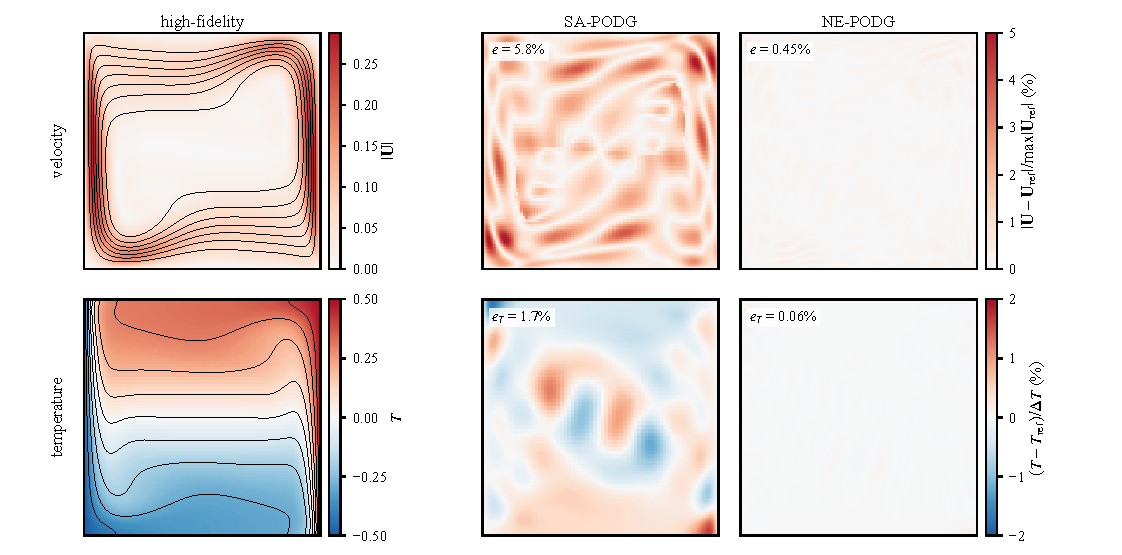
\includegraphics[width=\textwidth]{Fig_04.pdf}
\caption{快照预算 $N_{12}$ 下外推工况 $Ra=10^6$、$Pr=0.562$ 的高保真速度大小（附流线）与温度（附等温线），以及 SA-PODG 与 NE-PODG 的速度误差 $|\mathbf U-\mathbf U_{\mathrm{ref}}|/\max|\mathbf U_{\mathrm{ref}}|$ 与温度误差 $(T-T_{\mathrm{ref}})/\Delta T$，超出色标范围的取端色。各图左上角为该方法的速度误差 $e$ 与温度误差 $e_T$。}
\label{fig:contours}
\end{figure}

\begin{figure}[H]
\centering
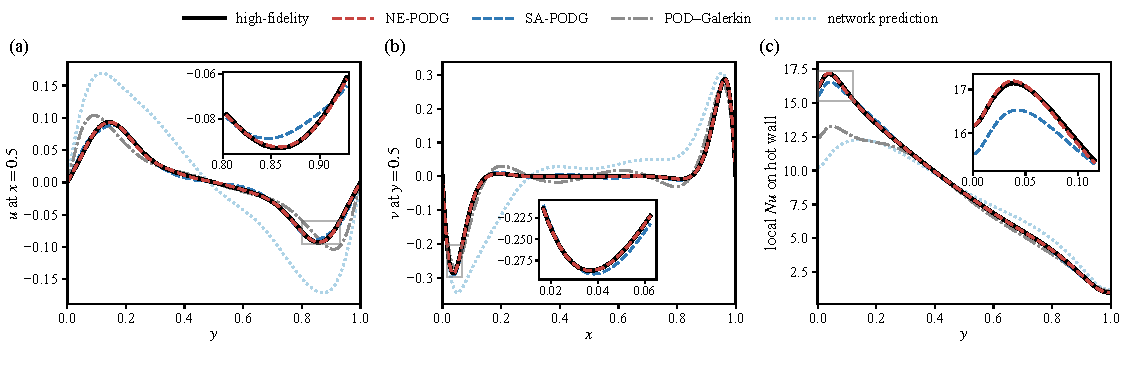
\includegraphics[width=\textwidth]{Fig_05.pdf}
\caption{快照预算 $N_{12}$ 下外推工况 $Ra=10^6$、$Pr=0.562$ 的 (a) $x=0.5$ 处水平速度 $u$ 沿 $y$ 的分布、(b) $y=0.5$ 处竖直速度 $v$ 沿 $x$ 的分布与 (c) 热壁局部 Nusselt 数。网络预测为网络输出 $\hat{\mathbf q}_\theta=\Phi_\theta w_\theta$ 及由其速度求得的温度；小图为方框区域的放大。}
\label{fig:fields}
\end{figure}

图~\ref{fig:contours} 与图~\ref{fig:fields} 给出方腔自然对流外推工况 $Ra=10^6$、$Pr=0.562$ 的场与剖面。SA-PODG 的速度误差分布在竖壁边界层与核心区，主场误差为 5.80\%；温度误差集中在核心区的分层结构上，为 1.68\%。NE-PODG 的速度与温度误差在全场都很小，主场误差为 0.853\%，温度误差为 0.105\%。中线速度剖面上，SA-PODG 在近壁峰值处偏离高保真解，NE-PODG 与之重合；热壁局部 Nusselt 数的峰值位于热壁底部，SA-PODG 在峰值附近偏低，NE-PODG 与高保真解一致，平均 Nusselt 数误差由 0.763\% 降为 0.0013\%。

\begin{figure}[H]
\centering
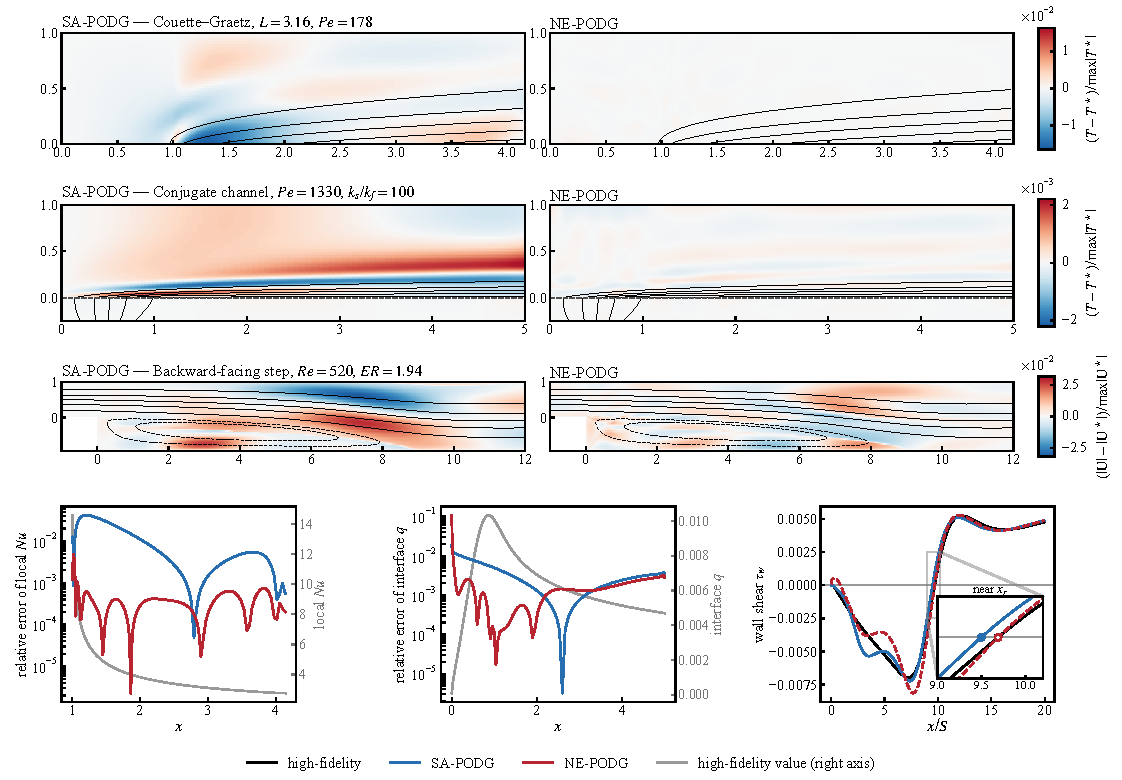
\includegraphics[width=\textwidth]{Fig_06.pdf}
\caption{Couette--Graetz（$L=3.16$、$Pe=178$）、共轭传热（$Pe=1330$、$k_s/k_f=100$）与后台阶（$Re=520$、$ER=1.94$）外推工况的场与壁面传热，各取 SA-PODG 误差最接近外推中位数的工况。前三行为 SA-PODG 与 NE-PODG 的有符号误差：温度为 $(T-T^\star)/\max|T^\star|$，后台阶为速度大小 $(|\mathbf U|-|\mathbf U^\star|)/\max|\mathbf U^\star|$，同一行两图色标相同；黑线为高保真解的等温线或流线（虚线为回流区流线），共轭传热中的水平虚线为流固界面。末行为沿壁面的相对误差：Couette--Graetz 与后台阶为受热壁局部 Nusselt 数，共轭传热为界面热流 $q$；灰线为高保真值（右轴）。}
\label{fig:fields_cases}
\end{figure}

图~\ref{fig:fields_cases} 给出另外三个算例的外推工况。Couette--Graetz 中，SA-PODG 的温度误差集中在受热段起点下游的热边界层内，受热壁局部 Nusselt 数的相对误差在受热段前部达到 $4\times10^{-2}$；NE-PODG 的温度误差在同一色标下几乎不可见，局部 Nusselt 数误差除受热段起点外低于 $10^{-3}$。共轭传热中，SA-PODG 的误差沿热边界层外缘形成条带并向下游增长；NE-PODG 去除了这一条带，界面热流的误差在入口段与加热段前部降低一到两个数量级，在下游与 SA-PODG 相当，约为 $3\times10^{-3}$。后台阶中，SA-PODG 的速度误差位于剪切层与再附着区附近；NE-PODG 降低了这部分误差，主场误差由 5.01\% 降为 2.87\%，主再附着长度 $x_r/S$ 为 9.688（高保真解 9.687，SA-PODG 9.496）。受热壁局部 Nusselt 数在再附着点上游变化剧烈，两种方法在该段的相对误差都在 $10^{-1}$ 量级。

\subsection{Mechanism of neural enrichment（神经增广的机制）}
\label{sec:mechanism}

\begin{figure}[H]
\centering
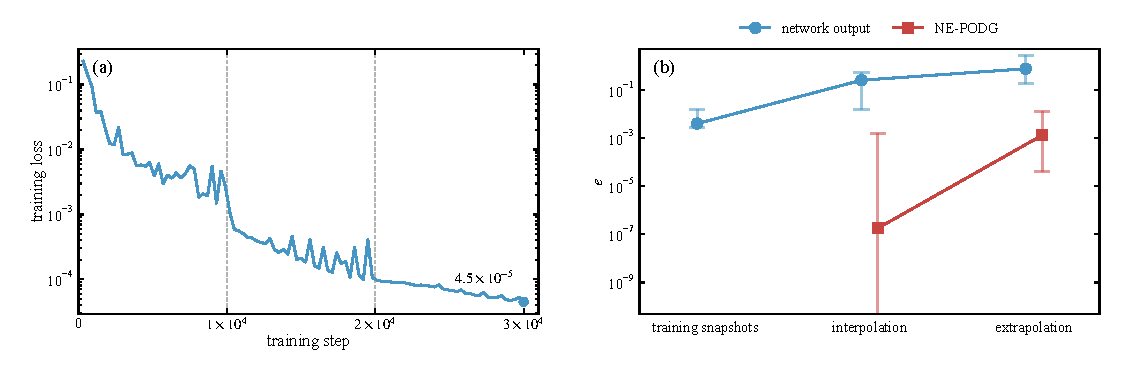
\includegraphics[width=\textwidth]{Fig_07.pdf}
\caption{快照预算 $N_{12}$ 下的网络。(a) 训练损失，虚线处学习率降为 1/10；(b) 网络直接输出 $\hat{\mathbf q}_\theta=\Phi_\theta w_\theta$ 与 NE-PODG 在训练快照、内插与外推工况上的速度误差 $e$，点为中位数，竖线为最小值到最大值。}
\label{fig:training}
\end{figure}

\begin{table}[H]
\centering
\caption{快照预算 $N_{12}$ 下网络直接输出 $\hat{\mathbf q}_\theta=\Phi_\theta w_\theta$ 与 NE-PODG 的误差（\%，中位数 / 最大值）。训练快照、内插与外推工况分别为 12、100、27 个；网络直接输出的温度由其速度在全网格上求解能量方程得到。}
\label{tab:network}
\small
\setlength{\tabcolsep}{3pt}
\begin{tabular}{llccc}
\toprule
工况 & 方法 & 速度 $e$ & 温度 $e_T$ & 平均 Nu \\
\midrule
训练快照 & 网络输出 & 0.23 / 0.81 & 0.0062 / 0.28 & $3.8\times10^{-4}$ / 0.033 \\
\midrule
\multirow{2}{*}{内插} & 网络输出 & 14.9 / 49.6 & 2.4 / 37.7 & 1.07 / 19.3 \\
 & NE-PODG & $1.2\times10^{-4}$ / 0.44 & $1.6\times10^{-6}$ / 0.057 & $2.8\times10^{-8}$ / 0.0052 \\
\midrule
\multirow{2}{*}{外推} & 网络输出 & 34.1 / 124 & 27.8 / 52.3 & 1.96 / 11.3 \\
 & NE-PODG & 0.21 / 2.1 & 0.022 / 0.40 & $1.1\times10^{-3}$ / 0.083 \\
\bottomrule
\end{tabular}
\end{table}

网络在训练快照上拟合准确，在未见参数处的直接输出误差较大（图~\ref{fig:training}，表~\ref{tab:network}）。方腔自然对流 $N_{12}$ 的训练快照上，网络直接输出的速度误差中位数为 0.23\%，在内插与外推工况上为 14.9\% 与 34.1\%；由同一网络构造互补空间后，NE-PODG 的误差中位数为 $1.2\times10^{-4}\%$ 与 0.21\%。Couette--Graetz 算例中，网络在 4 个训练快照上的误差中位数为 0.098\%，在内插与外推工况上为 65.0\% 与 39.7\%，NE-PODG 为 0.0483\% 与 0.0661\%。NE-PODG 的精度来自网络张成的候选空间与 Galerkin 闭合，网络在查询参数处的预测值不直接进入降阶解。

\begin{figure}[H]
\centering
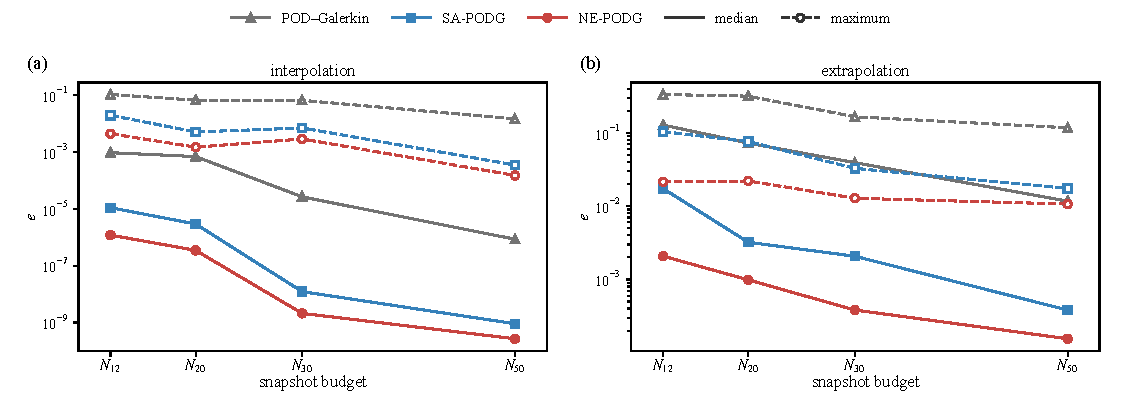
\includegraphics[width=\textwidth]{Fig_08.pdf}
\caption{神经增广的机制。(a) 方腔自然对流 $N_{12}$：SA-PODG 与未训练、训练网络（各三个种子合并）构造的 NE-PODG 的主场误差，上方数字为 $1-\Gamma_\theta$ 与 $\chi_B/\chi_W$ 的中位数；(b) 六个算例的 $1-\Gamma_\theta=(e_{\mathrm{proj},B}/e_{\mathrm{proj},W})^2$；(c) 六个算例的 $\chi_B/\chi_W$。细线为最小值到最大值，粗段为四分位区间，点为中位数（实心为内插，空心为外推）；$\times$ 为未收敛工况。(b)(c) 只含两种方法都解出且 $e_{\mathrm{proj},W}>10^{-9}$ 的工况。NC：方腔自然对流；CG：Couette--Graetz；CC：共轭传热；MC：混合对流；PC：多孔方腔；BFS：后台阶。}
\label{fig:mechanism}
\end{figure}

图~\ref{fig:mechanism}(a) 比较结构相同的训练与未训练网络。训练网络构造的增广空间使 $1-\Gamma_\theta$ 的中位数在内插与外推工况上为 0.014 与 0.037，未训练网络为 0.33 与 0.53；两者的 $\chi_B/\chi_W$ 中位数都在 0.99--1.08 之间。训练带来的误差下降来自余量捕获率的提高：训练网络的误差比 $e_{\mathrm{SA}}/e_{\mathrm{NE}}$ 中位数在三个种子上为 7.8--9.9（内插）与 5.3--6.1（外推），未训练网络为 1.7 与 1.3。

图~\ref{fig:mechanism}(b)(c) 给出六个算例的 $1-\Gamma_\theta$ 与 $\chi_B/\chi_W$。$1-\Gamma_\theta$ 的中位数在 Couette--Graetz 与共轭传热上为 $10^{-3}$ 量级，在方腔自然对流、混合对流与多孔方腔上为 0.01--0.05，在后台阶上为 0.16（内插）与 0.14（外推），与图~\ref{fig:accuracy}(b) 的增益次序一致。$\chi_B/\chi_W$ 随算子性质变化。三个方腔类算例的中位数在 0.97--1.08 之间，增广空间上 Galerkin 解相对最佳逼近的放大与 SA-PODG 相当。非对称线性算子上该比值可明显大于 1：Couette--Graetz 内插为 1.46，共轭传热内插与外推为 1.26 与 1.84；这两个算例的余量捕获率接近 1，最佳逼近误差的下降仍转化为一个数量级以上的实际误差下降。后台阶的 $\chi_B/\chi_W$ 中位数为 1.21 与 1.32，余量捕获率又最低，因而增益最小。由式~\eqref{eq:error_ratio}，$\ln(e_W/e_B)=-\tfrac12\ln(1-\Gamma_\theta)-\ln(\chi_B/\chi_W)$。逐工况比较两项的绝对值，前五个算例的全部工况、后台阶内插 100 个工况中的 95 个与外推 25 个工况中的 17 个，最佳逼近项大于闭合项。NE-PODG 的精度收益主要来自神经互补空间对余量的捕获；后台阶外推中，闭合放大的变化对部分工况的收益有相当的影响。

\subsection{Enrichment dimension and snapshot budget（增广维数与快照预算）}
\label{sec:dimension}
\label{sec:budget}

\begin{figure}[H]
\centering
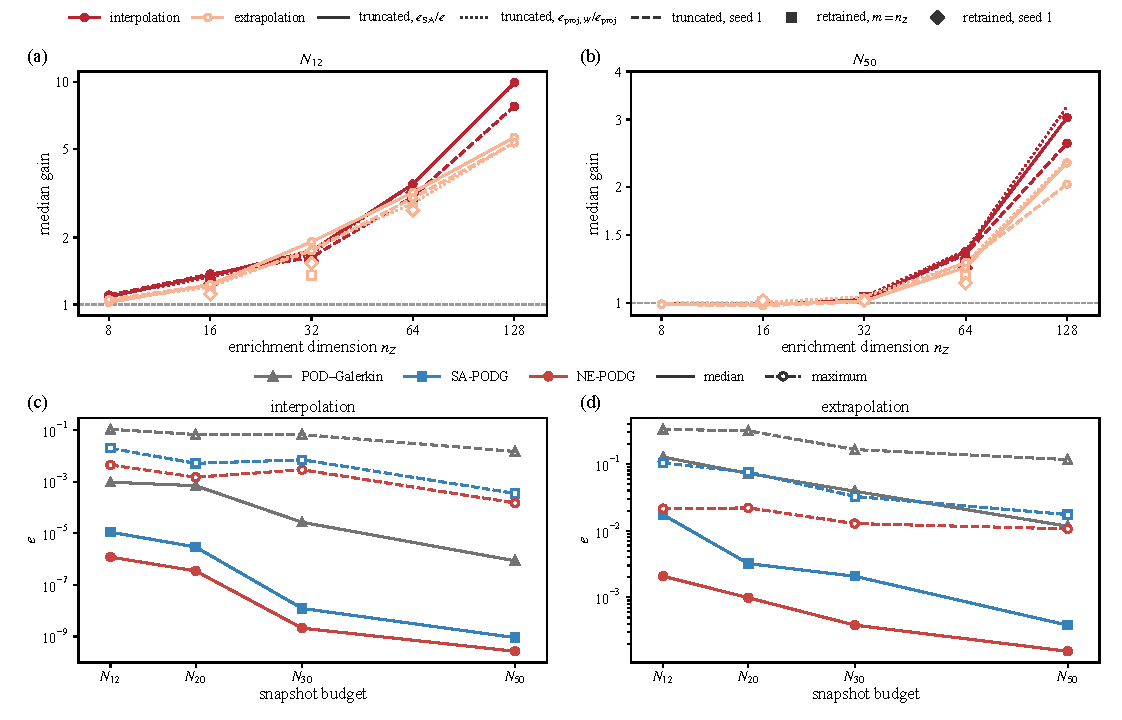
\includegraphics[width=\textwidth]{Fig_09.pdf}
\caption{方腔自然对流的增广维数与快照预算。(a) $N_{12}$、(b) $N_{50}$：逐工况增益中位数随增广维数 $n_Z$ 的变化，实线为求解误差比 $e_{\mathrm{SA}}/e$，点线为最佳逼近误差比 $e_{\mathrm{proj},W}/e_{\mathrm{proj}}$；圆点连线为把 $m=128$ 的网络截断到其候选场前 $n_Z$ 个奇异方向（实线种子 1234，虚线种子 1），方块与菱形为以 $m=n_Z$ 重新训练的网络（种子 1234 与 1）；深红实心为内插，浅红空心为外推。(c) 内插与 (d) 外推工况上三种方法速度误差的中位数（实线）与最大值（虚线）随快照预算的变化。}
\label{fig:dimension}
\label{fig:budget}
\end{figure}

增广维数决定互补空间的容量。把 $m=128$ 的网络截断到其候选场的前 $n_Z$ 个奇异方向后（图~\ref{fig:dimension}(a)(b)），$N_{12}$ 下 NE-PODG 相对 SA-PODG 的增益中位数在 $n_Z=8$、16、32、64、128 时依次为 1.08、1.35、1.74、3.48、9.93（内插）与 1.02、1.23、1.91、3.19、5.64（外推），最佳逼近误差比随维数同步增长。$N_{50}$ 的基础空间维数已达 88（$n_V=35$，$n_S=53$），$n_Z\le32$ 时增益接近 1，$n_Z=64$ 与 128 时为 1.36 与 3.04（内插）、1.24 与 2.32（外推）。以 $m=n_Z$ 重新训练的网络在同一维数下的增益与截断相当：$N_{12}$ 种子 1234 内插中，$n_Z=16$、32、64 时重训为 1.26、1.63、3.07，截断为 1.35、1.74、3.48；种子 1 时 $n_Z=64$ 重训为 3.19，截断为 3.06。增广维数可以由一次训练的网络截断得到，不需要为每个维数单独训练。

\begin{table}[H]
\centering
\caption{方腔自然对流四档快照预算下的温度误差 $e_T$ 与平均 Nusselt 数误差的中位数（\%），以及 $N_{12}$、$N_{50}$ 下 NE-PODG 在三个训练种子之间误差中位数的范围。速度误差见图~\ref{fig:budget}(c)(d)。}
\label{tab:budget}
\footnotesize
\setlength{\tabcolsep}{2pt}
\begin{tabular}{llcccccc}
\toprule
 & & \multicolumn{3}{c}{Interpolation} & \multicolumn{3}{c}{Extrapolation} \\
\cmidrule(lr){3-5}\cmidrule(lr){6-8}
Budget & Error & POD-G & SA-PODG & NE-PODG & POD-G & SA-PODG & NE-PODG \\
\midrule
$N_{12}$ & $e_T$ & 0.00502 & $4.10\times10^{-5}$ & $1.59\times10^{-6}$ & 5.60 & 0.404 & 0.0215 \\
 & $\overline{Nu}$ & $2.60\times10^{-4}$ & $3.49\times10^{-6}$ & $2.84\times10^{-8}$ & 2.84 & 0.0792 & 0.00106 \\
\midrule
$N_{20}$ & $e_T$ & 0.00420 & $6.09\times10^{-6}$ & $3.52\times10^{-7}$ & 2.29 & 0.0915 & 0.0123 \\
 & $\overline{Nu}$ & $4.11\times10^{-4}$ & $2.27\times10^{-6}$ & $1.53\times10^{-8}$ & 1.02 & 0.00630 & $3.05\times10^{-4}$ \\
\midrule
$N_{30}$ & $e_T$ & $1.46\times10^{-4}$ & $2.62\times10^{-8}$ & $2.60\times10^{-9}$ & 0.993 & 0.0372 & 0.00465 \\
 & $\overline{Nu}$ & $2.78\times10^{-5}$ & $1.93\times10^{-9}$ & $1.15\times10^{-10}$ & 0.212 & 0.00707 & $2.73\times10^{-4}$ \\
\midrule
$N_{50}$ & $e_T$ & $2.18\times10^{-6}$ & $9.57\times10^{-10}$ & $2.39\times10^{-10}$ & 0.254 & 0.00343 & 0.00150 \\
 & $\overline{Nu}$ & $2.12\times10^{-7}$ & $5.07\times10^{-11}$ & $1.42\times10^{-11}$ & 0.0206 & $2.81\times10^{-4}$ & $7.54\times10^{-5}$ \\
\midrule
\multicolumn{8}{l}{NE-PODG, seeds 1234 / 1 / 2 (min--max of the medians)} \\
$N_{12}$ & $e$ & \multicolumn{3}{c}{$1.19\times10^{-4}$--$1.51\times10^{-4}$} & \multicolumn{3}{c}{0.208--0.227} \\
 & $e_T$ & \multicolumn{3}{c}{$1.59\times10^{-6}$--$2.21\times10^{-6}$} & \multicolumn{3}{c}{0.0215--0.0267} \\
 & $\overline{Nu}$ & \multicolumn{3}{c}{$2.84\times10^{-8}$--$5.34\times10^{-8}$} & \multicolumn{3}{c}{0.00106--0.00154} \\
$N_{50}$ & $e$ & \multicolumn{3}{c}{$2.47\times10^{-8}$--$3.61\times10^{-8}$} & \multicolumn{3}{c}{0.0155--0.0176} \\
 & $e_T$ & \multicolumn{3}{c}{$2.13\times10^{-10}$--$3.50\times10^{-10}$} & \multicolumn{3}{c}{0.00144--0.00167} \\
 & $\overline{Nu}$ & \multicolumn{3}{c}{$1.00\times10^{-11}$--$2.48\times10^{-11}$} & \multicolumn{3}{c}{$7.54\times10^{-5}$--$1.26\times10^{-4}$} \\
\bottomrule
\end{tabular}

\end{table}

快照预算增加时三种方法的误差都下降，NE-PODG 相对 SA-PODG 的增益随之减小（图~\ref{fig:budget}(c)(d)）：误差比中位数在 $N_{12}$、$N_{20}$、$N_{30}$、$N_{50}$ 下为 9.93、9.90、4.25、3.04（内插）与 5.64、4.25、2.56、2.32（外推）。快照稀疏时 NE-PODG 的优势最大：$N_{12}$ 的 NE-PODG 外推误差中位数为 0.208\%，与 $N_{30}$ 的 SA-PODG（0.207\%）相当。温度与平均 Nusselt 数的误差随预算的变化与速度误差总体一致（表~\ref{tab:budget}）。三个训练种子之间，NE-PODG 的误差中位数在 $N_{12}$ 外推中为 0.208\%--0.227\%，在 $N_{50}$ 外推中为 0.0155\%--0.0176\%，内插速度误差中位数的最大与最小值之比不超过 1.5。
